\documentclass[12pt]{article}
\usepackage[a4paper, total={6in, 9in}]{geometry}
\usepackage{graphicx}
\graphicspath{ {./images/output/} }
\usepackage{caption}
\usepackage[english]{babel}
\usepackage{titling}
\usepackage{float}
% \usepackage{amsmath}
% \usepackage{minted}
% \usepackage{multicol}
% \usepackage{array}
% \usepackage{setspace}
% \usepackage{placeins}

% \usepackage{lipsum}

\title{Single Phase Half Wave Rectifier Using Diode with R, RL Load}
\author{}
\date{}

\pagenumbering{gobble}
\begin{document}
% \vspace*{\fill}
\begin{center}

    \emph{Heaven's Light is Our Guide} \\
    \textbf{Rajshahi University of Engineering and Technology} \\

    \begin{figure}[H]
        \centering
        
\includegraphics[scale=.34]{images/RUET_logo.png}
        \label{fig:ruet_logo}
    \end{figure}
    \vspace{5mm}

    \textbf{Course Code}\\
    ECE 3206\\
    \vspace{3mm}
    \textbf{Course Title}\\
    Industrial Electronics Sessional

    \vspace{5mm}
    \textbf{Experiment Date:} {January 13, 2025},\\
    \textbf{Submission Date:} {February 10, 2025}\\

    \vspace{5mm}
    \textbf{Lab Report 3: \\
        Study of Thyristor Characteristics R, RL Load}

    \vspace{15mm}

    \begin{tabular}{c|c}
        \textbf{Submitted to} & \textbf{Submitted by} \\
        Md. Faysal Ahamed     & Md. Tajim An Noor     \\
        Lecturer              & Roll: 2010025         \\
        Dept of ECE, Ruet     &                       \\
    \end{tabular}

\end{center}
\vspace*{\fill}


\pagebreak

% \tableofcontents

\pagebreak
\pagenumbering{arabic}
\maketitle

\section*{Objective}
\addcontentsline{toc}{section}{Objective}
\begin{itemize}
    \item To use diodes to construct a half-wave rectifier.
    \item To perform the experiment using a diode testing kit.
    \item To learn and understand the operation of the diode testing kit.
\end{itemize}

\section*{Circuit Diagrams}
\addcontentsline{toc}{section}{Circuit Diagrams}
\begin{figure}[H]
    \centering
    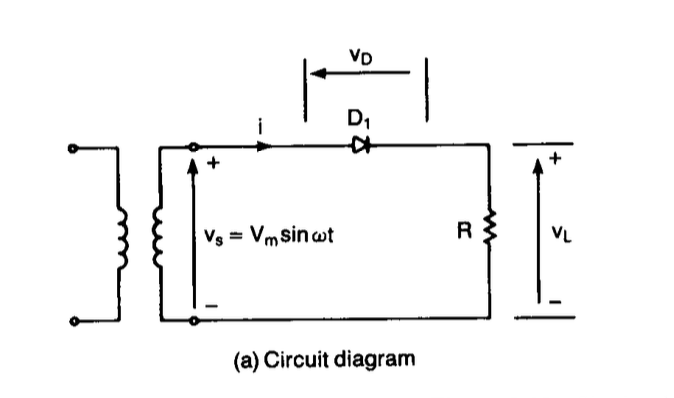
\includegraphics[width=.7\textwidth]{half_ckt.png}
    \caption{Diode Rectifier Circuit \cite{rashid2013power}}
    \label{fig:dc_r_load}
\end{figure}

\section*{Observations}
\addcontentsline{toc}{section}{Observations}
\begin{itemize}
    \item Constructed a half-wave rectifier using a diode and testing kit.
    \item Analyzed waveforms for R and RL loads on an oscilloscope.
    \item Observed smoother transitions and delays in RL load due to inductance.
    \item Confirmed diode's unidirectional conduction, blocking negative half-cycles.
\end{itemize}

\subsubsection*{Outputs}
\begin{figure}[H]
    \centering
    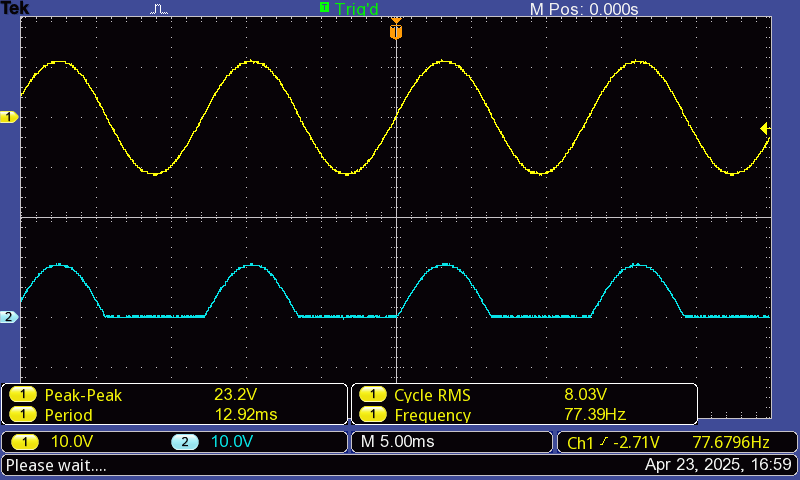
\includegraphics[width=.7\textwidth]{half_r_load3.png}
    \caption{Half wave rectifier output for R load}
    \label{fig:rLoad}
\end{figure}

\begin{figure}[H]
    \centering
    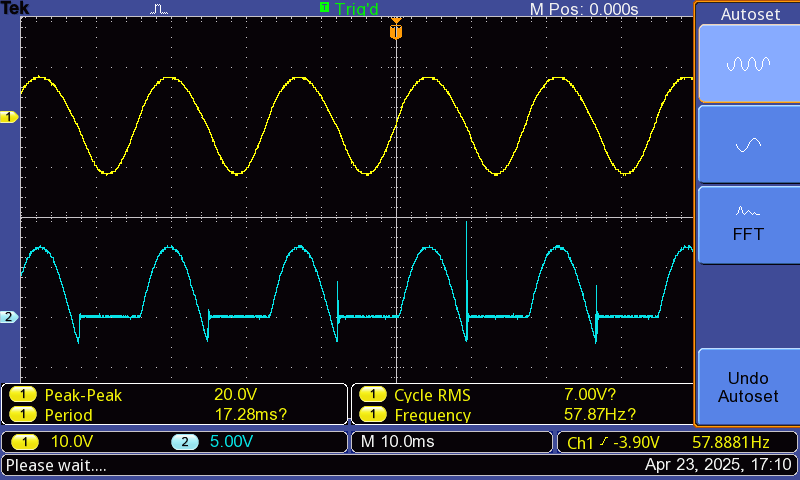
\includegraphics[width=.7\textwidth]{half_rl_load4.png}
    \caption{Half wave rectifier output for RL load}
    \label{fig:rLoadDelay}
\end{figure}

\bibliographystyle{IEEEtran}
\renewcommand{\bibname}{References}
\addcontentsline{toc}{section}{References}
\bibliography{ref}

\end{document}
